% Sybil attack flow (A5).
\documentclass[border=10pt,tikz]{standalone}
\usepackage{tikz}
\usetikzlibrary{arrows.meta,positioning,fit,calc,shapes.geometric}

\definecolor{sand}{HTML}{E9DCC4}
\definecolor{sanddeep}{HTML}{D4C5A9}
\definecolor{ebony}{HTML}{1E1B18}
\definecolor{ink}{HTML}{2C2A26}
\definecolor{cinnabar}{HTML}{CC3D2E}
\definecolor{brass}{HTML}{B08D57}
\definecolor{patina}{HTML}{5C7A6A}
\definecolor{paper}{HTML}{FBF7EE}

\begin{document}
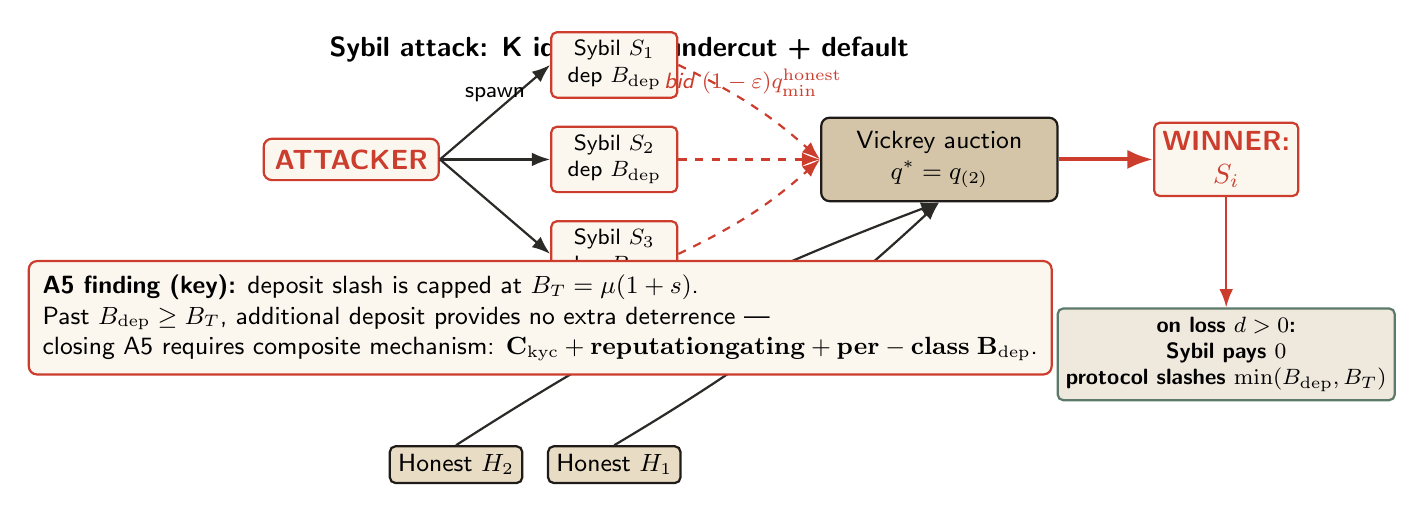
\begin{tikzpicture}[
  font=\sffamily\small,
  adv/.style={draw=cinnabar,thick,fill=paper,rounded corners=3pt,
              inner sep=4pt,minimum width=22mm,align=center,
              font=\sffamily\bfseries,text=cinnabar},
  sybil/.style={draw=cinnabar,thick,fill=paper,rounded corners=2pt,
                inner sep=3pt,minimum width=16mm,align=center,
                font=\sffamily\footnotesize},
  honest/.style={draw=ebony,thick,fill=sand,rounded corners=2pt,
                 inner sep=3pt,minimum width=16mm,align=center},
  auction/.style={draw=ebony,thick,fill=sanddeep,rounded corners=3pt,
                  inner sep=5pt,align=center,minimum width=30mm},
  payout/.style={draw=patina,thick,fill=paper,rounded corners=2pt,
                 inner sep=3pt,align=center,
                 font=\sffamily\footnotesize\bfseries},
  arr/.style={->,>=Latex,thick,draw=ink},
  badarr/.style={->,>=Latex,thick,draw=cinnabar,dashed},
]

\node[font=\sffamily\bfseries,anchor=west] at (-0.4,4.8)
  {Sybil attack: K identities, undercut + default};

% Attacker
\node[adv] (attacker) at (0,3.4) {ATTACKER};

% K Sybils
\node[sybil,right=14mm of attacker.east,yshift=12mm] (s1)
  {Sybil $S_1$\\dep $B_{\mathrm{dep}}$};
\node[sybil,right=14mm of attacker.east,yshift=0mm] (s2)
  {Sybil $S_2$\\dep $B_{\mathrm{dep}}$};
\node[sybil,right=14mm of attacker.east,yshift=-12mm] (s3)
  {Sybil $S_3$\\dep $B_{\mathrm{dep}}$};

\draw[arr] (attacker.east) -- node[above,font=\sffamily\footnotesize]
  {spawn} (s1.west);
\draw[arr] (attacker.east) -- (s2.west);
\draw[arr] (attacker.east) -- (s3.west);

% Honest insurers
\node[honest,below=18mm of s3.south,yshift=-2mm] (h1) {Honest $H_1$};
\node[honest,left=3mm of h1] (h2) {Honest $H_2$};

% Auction
\node[auction,right=18mm of s2] (auction) {Vickrey auction\\$q^* = q_{(2)}$};
\draw[badarr] (s1.east) to[bend left=8]
  node[above,font=\sffamily\footnotesize\itshape,text=cinnabar]
  {bid $(1-\varepsilon) q_{\min}^{\mathrm{honest}}$} (auction.west);
\draw[badarr] (s2.east) to (auction.west);
\draw[badarr] (s3.east) to[bend right=8] (auction.west);
\draw[arr] (h1.north) to[bend right=6] (auction.south);
\draw[arr] (h2.north) to[bend left=6] (auction.south);

% Winner = Sybil (with high probability)
\node[draw=cinnabar,thick,fill=paper,rounded corners=2pt,inner sep=3pt,
      align=center,right=12mm of auction,font=\sffamily\bfseries,
      text=cinnabar] (winner) {WINNER:\\$S_i$};
\draw[arr,line width=1.4pt,draw=cinnabar] (auction.east) -- (winner.west);

% On loss: Sybil defaults; protocol confiscates deposit
\node[payout,below=14mm of winner,fill=brass!20]
  (lossbox) {on loss $d > 0$:\\Sybil pays $0$\\protocol slashes $\min(B_{\mathrm{dep}}, B_T)$};
\draw[arr,draw=cinnabar] (winner.south) -- (lossbox.north);

% Coverage ceiling callout
\node[draw=cinnabar,thick,fill=paper,rounded corners=3pt,inner sep=5pt,
      align=left,minimum width=100mm,below=10mm of attacker.south,xshift=24mm]
  {{\bfseries A5 finding (key):} deposit slash is capped at $B_T = \mu(1 + s)$.\\
   Past $B_{\mathrm{dep}} \geq B_T$, additional deposit provides no extra
   deterrence — \\
   closing A5 requires composite mechanism:
   $\mathbf{C_{\mathrm{kyc}} + \text{reputation gating} +
   \text{per-class}\; B_{\mathrm{dep}}}$.};

\end{tikzpicture}
\end{document}
